\documentclass[a4paper, czech]{article}

\title{Úloha č.3: Elektronkový zesilovač - Simulace}
\author{Karolína Andrea Šebestová}
\date{Datum měření: 21.10.2024}

\usepackage[czech]{babel}
%\usepackage[T1]{fontenc}
\usepackage{indentfirst}
\usepackage{graphicx}
\usepackage{float}
\usepackage[margin=1.5cm]{geometry}
\usepackage{booktabs}
\usepackage{amsmath}
\usepackage{caption}
\usepackage{subcaption}

\begin{document}

\maketitle

\begin{figure}[H]
    \centering
    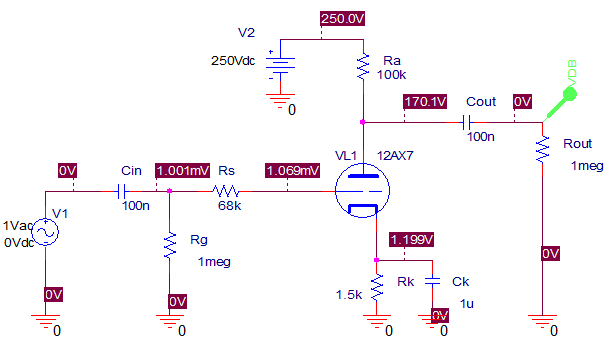
\includegraphics[width=0.7\textwidth]{schema.png}
\end{figure}

\section{Úkoly měření}

\begin{enumerate}
    \item V tomto úkolu se seznámíte s převodní charakteristikou elektronkové triody, což je závislost anodového (výstupního) proudu na (vstupním) napětí na mřížce. Otevřete projekt Prevodni char a prohlédněte si schéma. V menu PSpice, Edit Simulation Profile si prohlédněte nastavení simulace. Půjde o stejnosměrnou analýzu (DC Sweep) se změnou napětí zdroje V1 od -3 do 0 V s krokem 0,1 V. Toto nastavení neměňte (zvolte Storno) a spusťte simulaci z menu PSpice, Run (zkratková klávesa F11). V novém okně by se měla vykreslit požadovaná převodní charakteristika. Tuto charakteristiku vložte do protokolu a okomentujte ji. Zamyslete se nad vhodnou volbou pracovního bodu elektronkového zesilovače, tedy pro jaká vstupní napětí je převodní charakteristika lineární a nedojde ke zkreslení či limitaci.
    \item Nyní se budeme zabývat výstupními charakteristikami triody, tedy závislostmi výstupního proudu na napětí mezi anodou a katodou. Parametrem křivek bude napětí na mřížce. Otevřete projekt Vystupni char a prohlédněte si schéma. V menu PSpice, Edit Simulation Profile si prohlédněte nastavení simulace. Půjde opět o stejnosměrnou analýzu se změnou napětí zdroje V2 od 0 do 250 V s krokem 10 V. V tomto případě je ještě aktivována parametrická analýza (Parametric Sweep). Po kliknutí na její nastavení (vlevo v okně Options) lze vidět, že se jako parametr bude měnit napětí zdroje V1, a to od -3 do 0 V po 0,2 V. Toto nastavení opět neměňte a spusťte simulaci. Charakteristiky opět vložte do protokolu a slovně popište jejich význam.
    \item Zde bude simulována závislost přenosu (zesílení) celého zesilovače s triodou na kmitočtu. Otevřete projekt Zesilovac AC char a prohlédněte si schéma. V menu PSpice, Edit Simulation Profile si prohlédněte nastavení simulace. Je aktivována analýza AC Sweep, tedy střídavá analýza zobrazující frekvenční charakteristiky. Všimněte si rozsahu kmitočtu. Spusťte simulaci, výslednou charakteristiku vložte do protokolu a zhodnoťte ji. Změňte hodnotu Rs (např. na pětinásobek a na pětinu původní hodnoty) a zhodnoťte vliv na průběh zesílení. Podobně zjistěte také vliv změny Ck, Cin a Cout na průběh zesílení (měňte uvedené kapacity jednotlivě).
    \item V tomto úkolu budou simulovány časové průběhy signálů v obvodu. Otevřete projekt Zesilovac transient a prohlédněte si schéma. V menu PSpice, Edit Simulation Profile si prohlédněte nastavení simulace. Je aktivována analýza Time Domain (Transient), tedy časová analýza. Všimněte si parametru Run to time znamenajícího časový rozsah simulace. Spusťte simulaci, výslednou charakteristiku vložte do protokolu a zhodnoťte ji. Změňte amplitudu vstupního signálu (parametr VAMPL zdroje V1). Nastavte ji na 2 V, kdy by mělo dojít ve výstupním signálu k limitaci, což ověřte. Na základě převodní charakteristiky vysvětlete příčinu limitace jak v kladné, tak v záporné půlvlně výstupního signálu. Oba průběhy, tedy s limitací a bez, vložte do protokolu.
    \pagebreak
    \item Pomocí tlačítka FFT v okně grafických charakteristik zobrazte spektrum výstupního signálu při vstupní amplitudě 2 V. Vypočítejte harmonické zkreslení (THD - Total Harmonic Distortion) podle prvních 20-ti harmonických složek podle vztahu:
    \begin{equation*}
        THD = \sqrt{\frac{U_2^2 + U_3^2 + ... + U_{20}^2}{U_1^2 + U_2^2 + ... + U_{20}^2}} \cdot 100 \%
    \end{equation*}
    kde $U_1$ je amplituda (velikost spektrální čáry) první harmonické složky o frekvenci $f_{in}$ = 1,5 kHz, $U_2$ je amplituda následující složky o frekvenci $2 f_{in}$, $U_3$ je amplituda složky o frekvenci $3f_{in}$ atd. Při odečítání velikostí jednotlivých harmonických složek používejte kurzory a vhodně měňte měřítka os dvojklikem na osy nebo tlačítky. Zjistěte, jak bude znít zvuk s takovouto hodnotou THD.
\end{enumerate}

\section{Zpracování úkolů}

\subsection{Úkol měření 1)}

V tomto úkolu jsme realizovali simulaci samotné elektronkové triody, jíž výsledkem je její převodní charakteristika.
Jedná se o závislost anodového (výstupního) proudu na (vstupním) napětí na mřížce.

\begin{figure}[H]
    \centering
    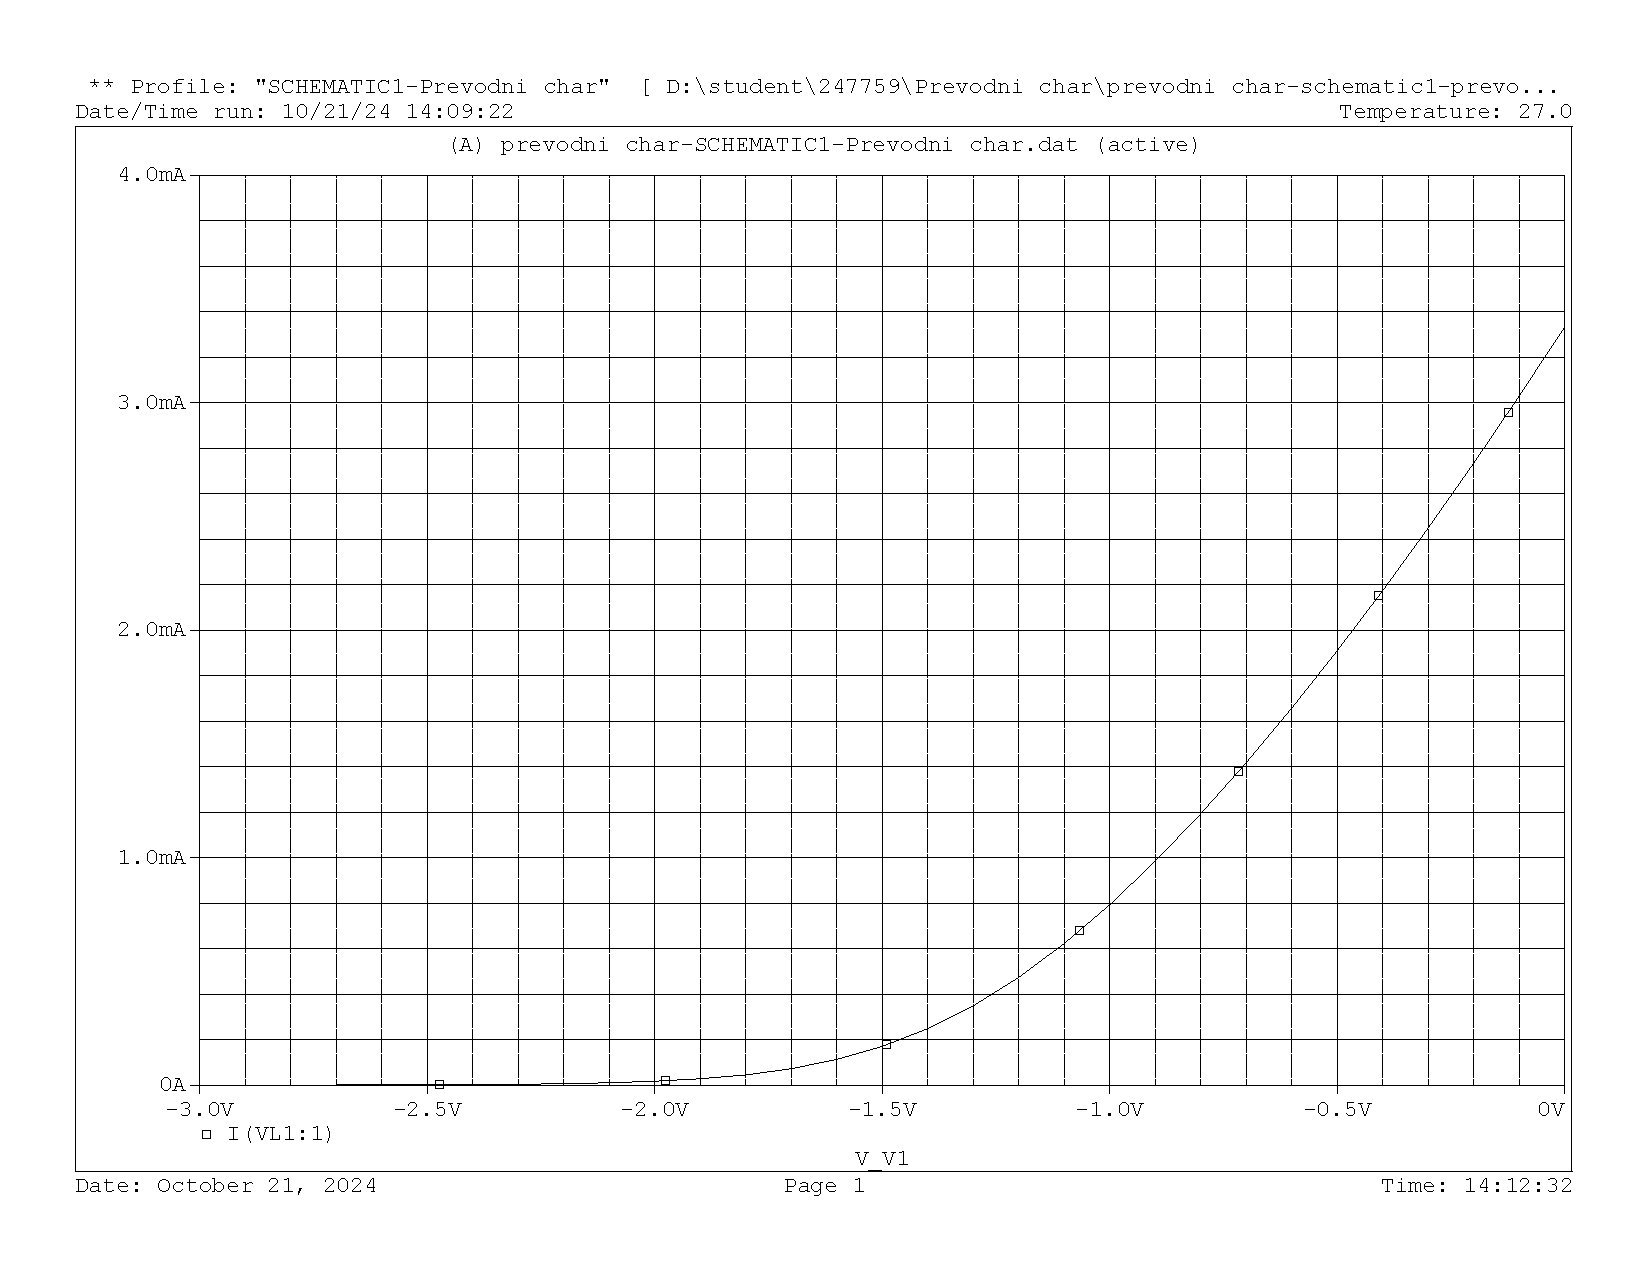
\includegraphics[width=\textwidth]{charakteristiky/ULOHA1.pdf}
    \caption{Převodní charakteristika elektronkové triody}
\end{figure}

Tuto převodní charakteristiku nelze považovat za lineární, jedná se spíše o exponenciální průběh.
Pozorujeme, že v první třetině napěťového rozsahu na mřížce (t.j. od -3 do cca. -2V) lze výstupní proud na anodě považovat za téměř nulový.
Tento jev je způsoben záporně nabitou mřížkou triody, která odpuzuje elektrony kolem ní prolétávající od katody k anodě elektronky a brání tak toku proudu.
Triodu lze na tomto rozsahu považovat za uzavřenou, analogicky k tranzistoru, neboli spíše k vodovodnímu (elektronovému) kohoutku.

Ve druhé třetině napěťového rozsahu na mřížce (t.j. cca. od -2 do cca. -1V) začíná docházet k přechodu od uzavřeného do otevřeného stavu triody.
Tento přechod však není lineární a při použití elektronky v zesilovači by v této oblasti docházelo k vysokému zkreslení.

V poslední třetině charakteristiky (t.j. od cca. -2 do 0V) se již jedná o téměř lineární průběh, který je vhodný pro umístění pracovního bodu elektronkového zesilovače.
V případě použití této elektronky v zesilovači třídy A by bylo vhodné pracovní bod umístit do středu tohoto rozsahu, t.j. přibližně na hodnotu 0,5V.
Bylo by však potřebné zajistit, aby rozkmit vstupního signálu nikdy nepřesáhl hodnotu 0V, kde by docházelo k limitaci signálu, a také neklesl pod hodnotu -1V, kde je charakteristika nelineární a docházelo by zde ke zkreslení a v případě velkého poklesu až do oblasti, kde je elektronka uzavřená, také k limitaci.

\subsection{Úkol měření 2)}

V této úloze jsme se opět věnovali simulaci elektronkové triody.
Výsledkem simulace je tentokrát však soubor výstupních charakteristik triody.
Jedná se o závislost výstupního proudu na napětí mezi anodou a katodou.
Jednotlivé křivky se od sebe liší velikostí napětí přivedeného na mřížku elektronky. 

\begin{figure}[H]
    \centering
    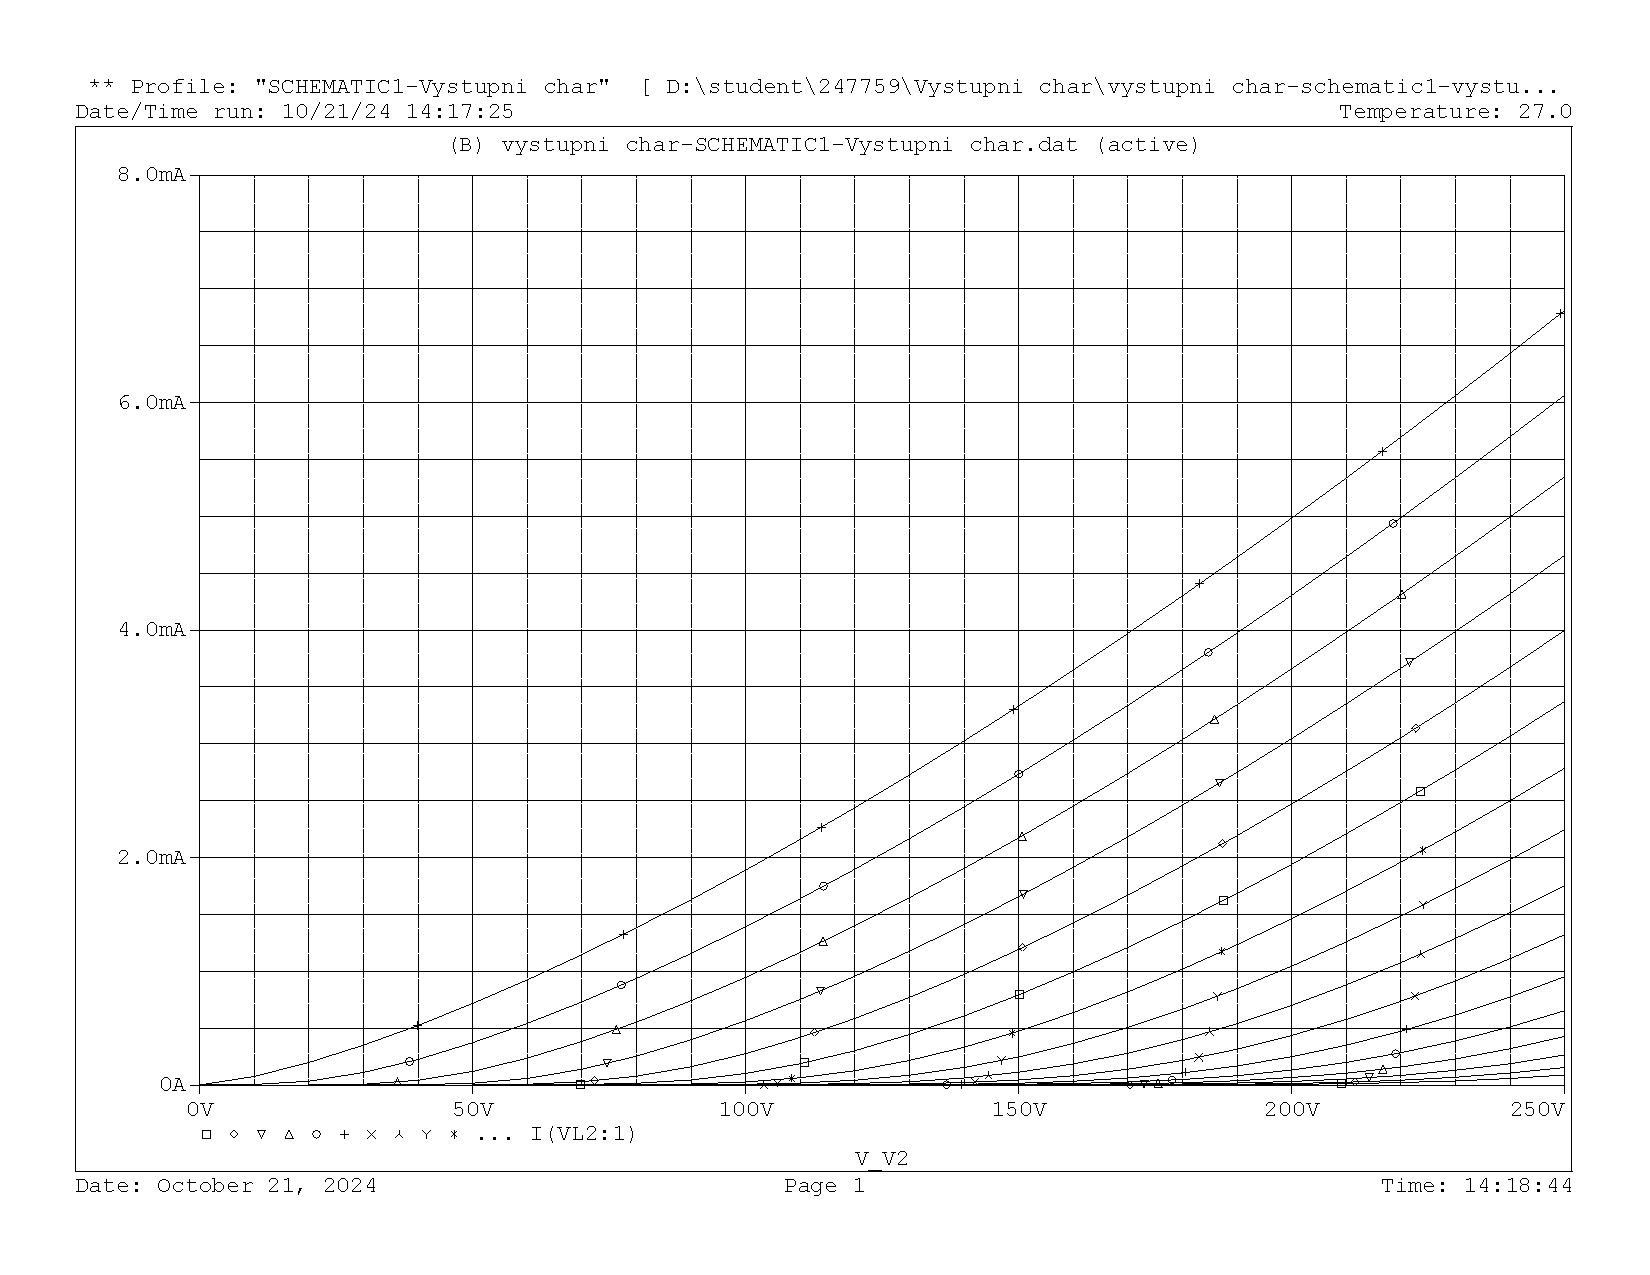
\includegraphics[width=\textwidth]{charakteristiky/uloha2.pdf}
    \caption{Výstupní charakteristiky triody}
\end{figure}

Pozorujeme stejný jev jako v předcházejícím úkolu, t.j. záporně nabitá mřížka diody odpuzuje elektrony proudu protékajícího elektronkou, čímž brání průtoku proudu.
Lépe řečeno, velikostí záporného napětí přivedeného na mřížku lze úměrně řídit velikost proudu protékajícího elektronkou.

První (vrchní) průběh ve výše uvedeném grafickém znázornění výstupních charakteristik je možné (s přihmouřenými oči nad začátkem průběhu) považovat za lineární.
Na dalších průbězích pozorujeme na jejich začátcích nulovou oblast, která se, se snižujícím se napětím na mřížce elektronky, prodlužuje.
Oblast průběhů, kdy proud začne stoupat, se postupně oddaluje od počátku charakteristiky.
Čím nižší napětí na mřížku elektronky přivedeme, tím větší proud je tedy schopna "odpudit".

\pagebreak

\subsection{Úkol měření 3)}

V tomto úkolu jsme se již věnovali simulacím celého elektronkového zesilovače.
Výsledkem těchto simulací jsou frekvenční charakteristiky zesilovače - závislost přenosu (zesílení) triodového zesilovače na kmitočtu vstupního signálu. 
Na následujícím obrázku je znázorněna frekvenční charakteristika zesilovače v jeho nezměněném stavu.
Následující obrázky v této sekci popisují vliv změn hodnot jednotlivých součástek obvodu na průběh charakteristiky. 

\begin{figure}[H]
    \centering
    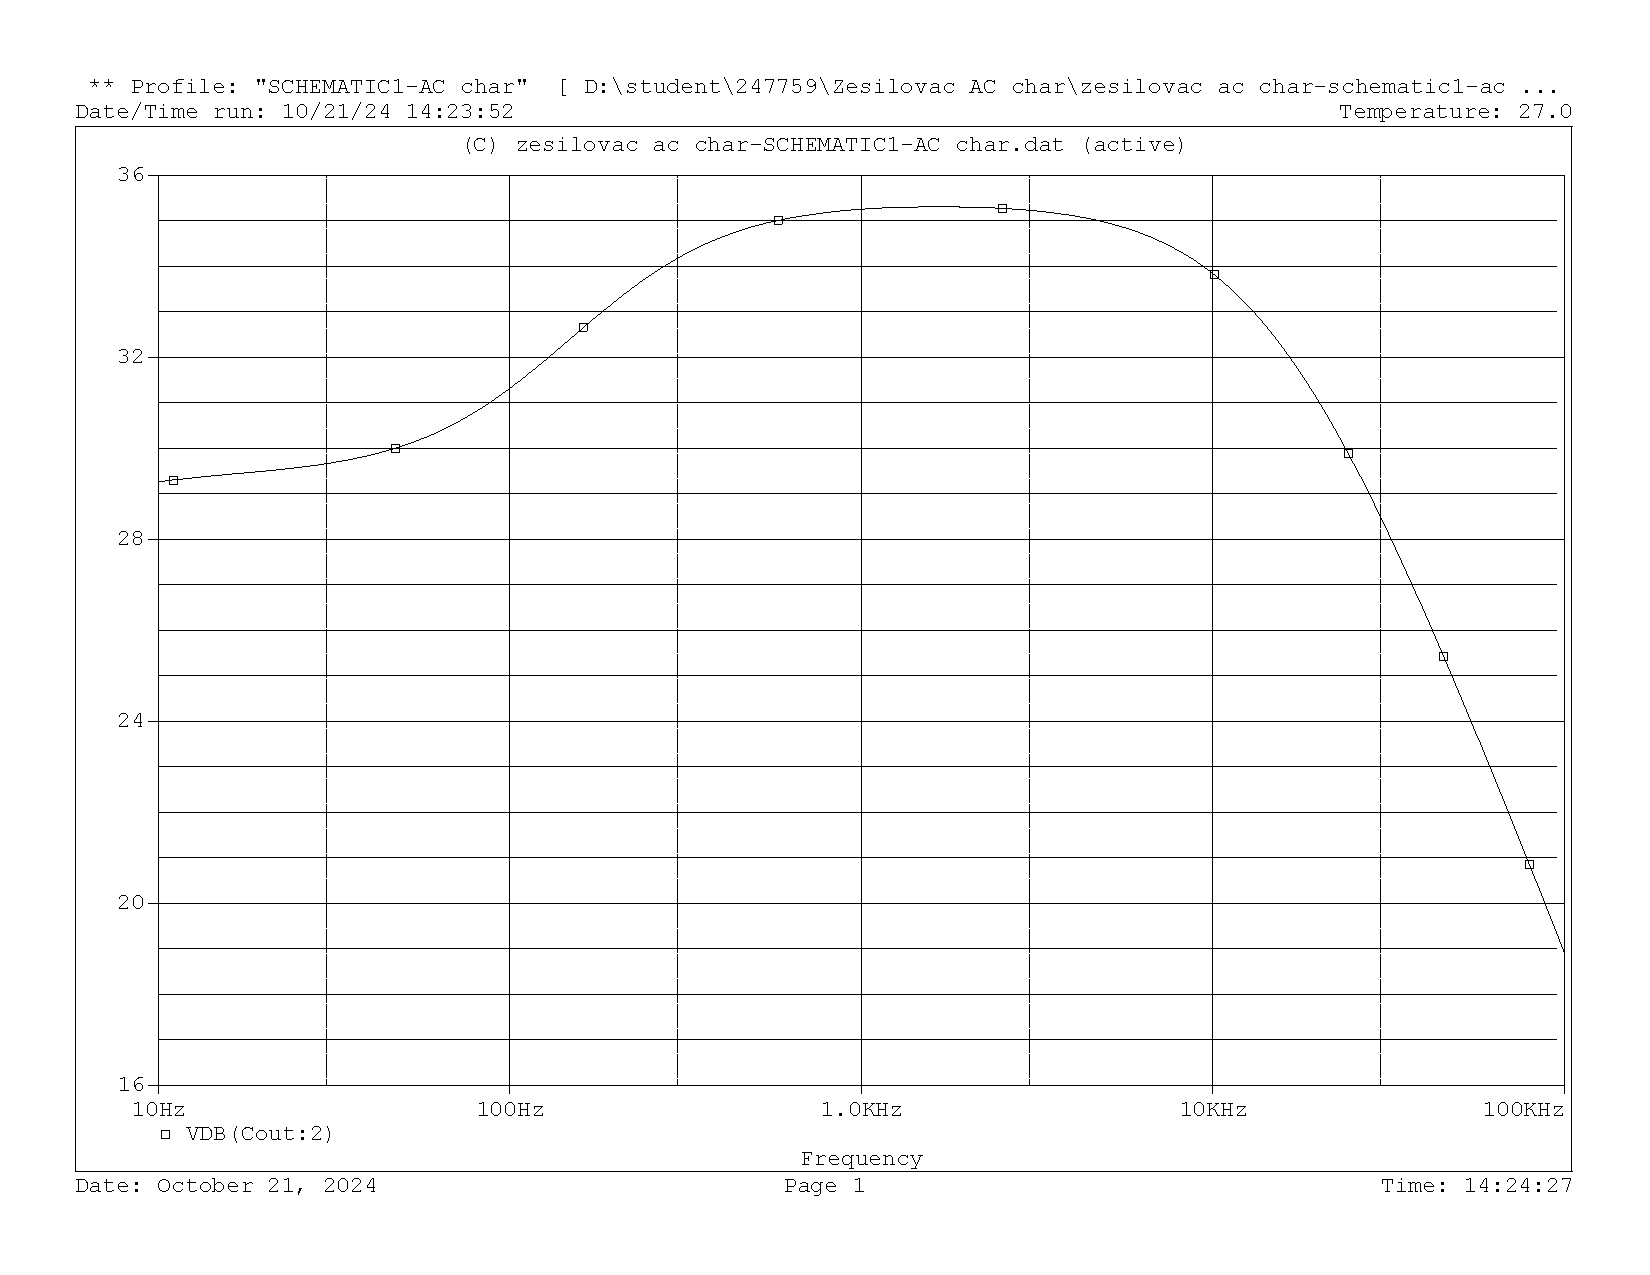
\includegraphics[width=\textwidth]{charakteristiky/uloha3.pdf}
    \caption{Frekvenční charakteristika celého zesilovače}
\end{figure}

Pozorujeme, že kmitočtová závislost přenosu zesilovače má charakter přibližně jako pásmová propust.
V nižších kmitočtech však nedochází k úplnému potlačení zesílení, pouze k jeho poklesu.
Tento jev je pravděpodobně způsoben vazebními kapacitory na vstupu a výstupu obvodu, ke kterým jsou paralelně připojeny rezistory a tvoří tak CR články. 
Ve vyšších kmitočtech již začíná docházet k úplnému potlačení.
To je nejspíše způsobeno tím, že omezující rezistor Rs na vstupu obvodu tvoří RC článek s Millerovou (vstupní) kapacitou vznikající mezi mřížkou a anodou použité triody.

\begin{figure}[H]
    \centering
    \begin{subfigure}{0.49\textwidth}
        \centering
        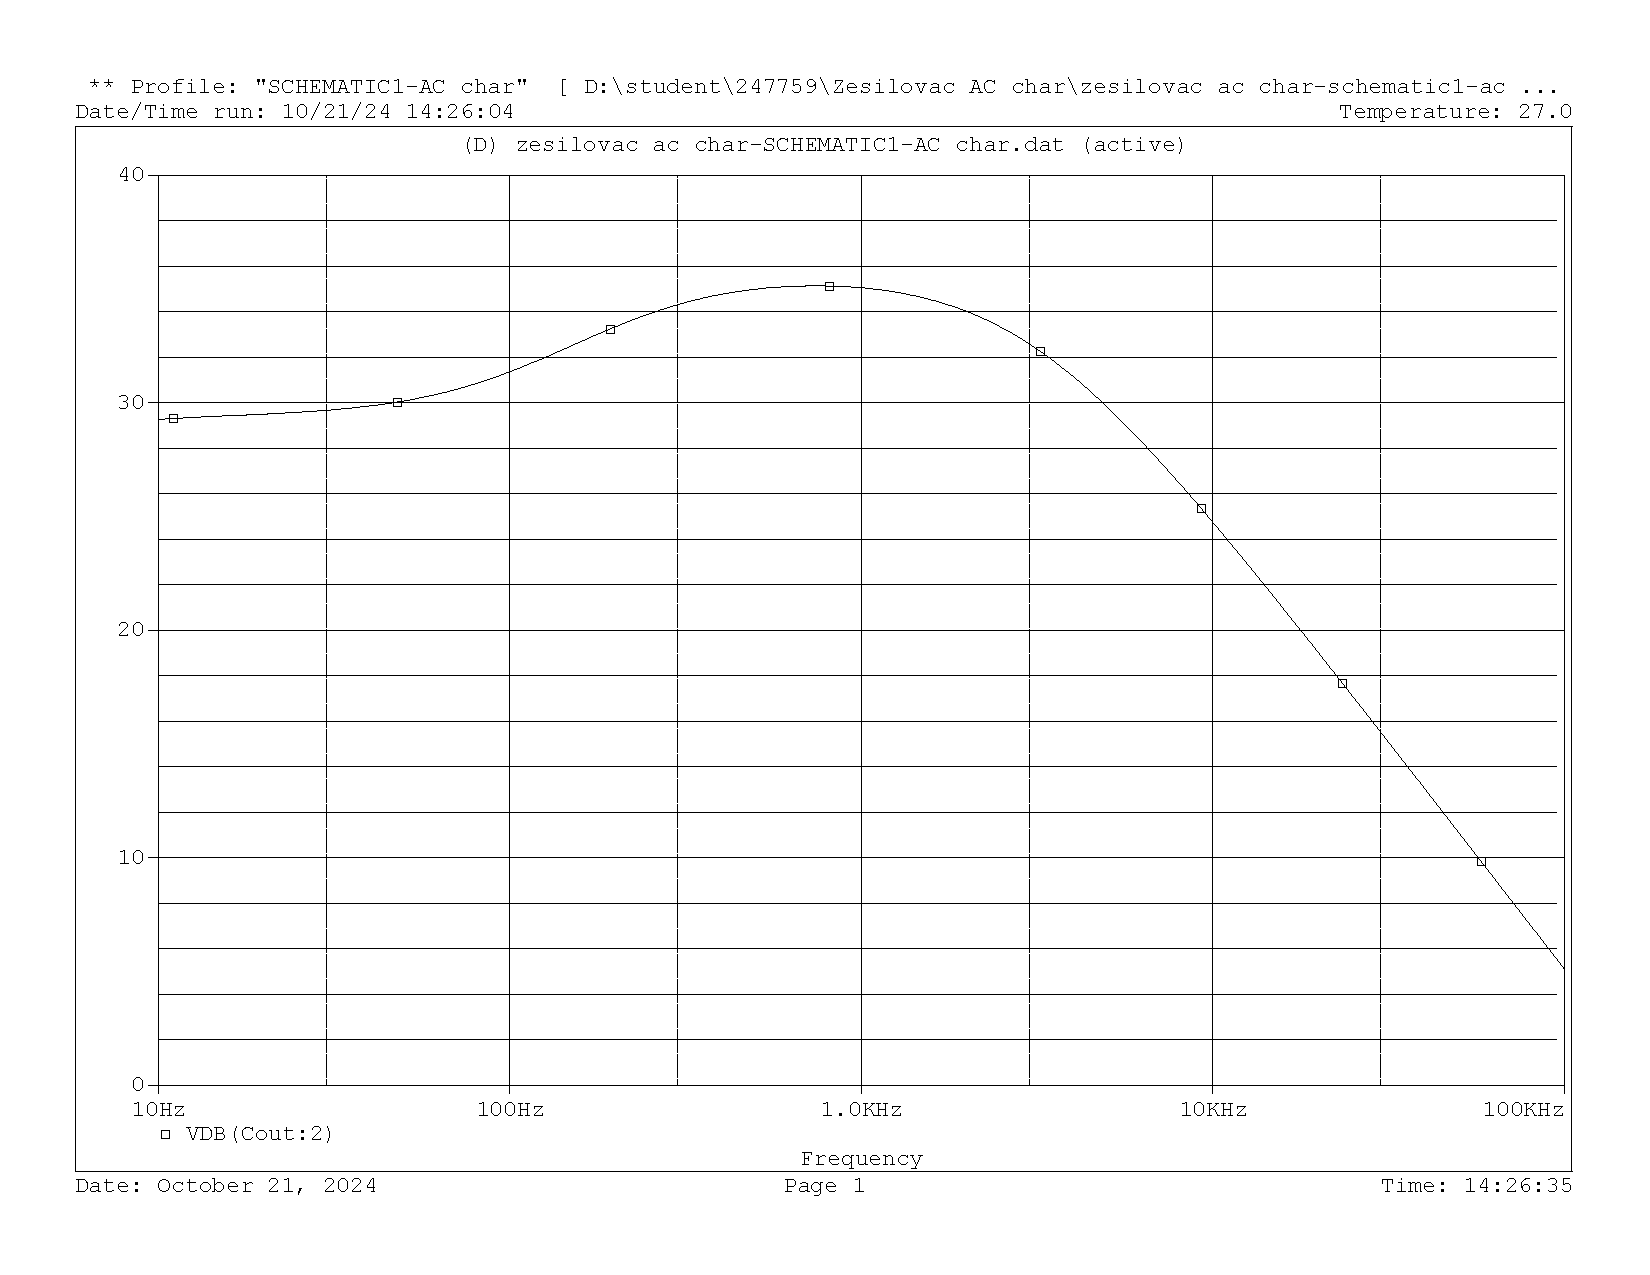
\includegraphics[width=\textwidth]{charakteristiky/uloha3_Rs_5krat_vetsi_340k.pdf}
        \caption{Pětinásobek původní hodnoty Rs (340 k$\Omega$)}
    \end{subfigure}
    \hfill
    \begin{subfigure}{0.49\textwidth}
        \centering
        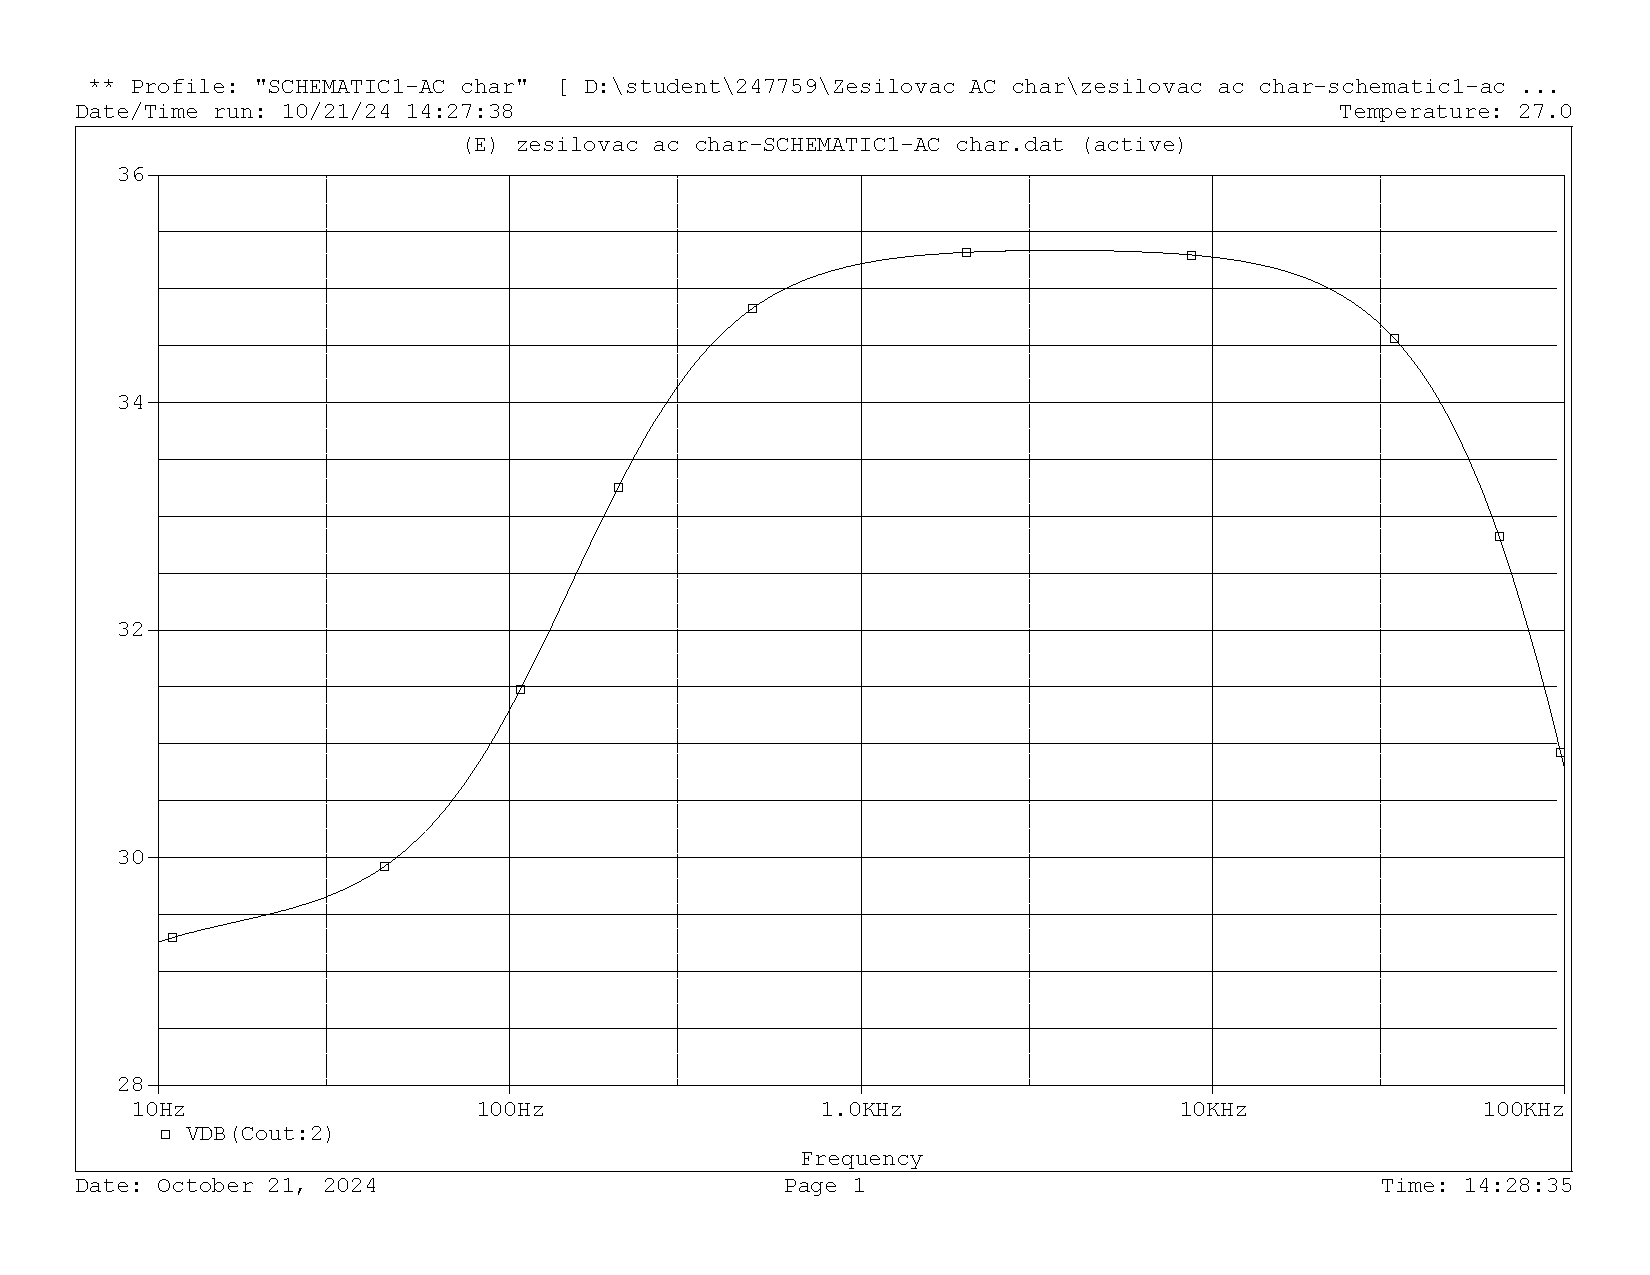
\includegraphics[width=\textwidth]{charakteristiky/uloha3_Rs_5krat_mensi_13_6k.pdf}
        \caption{Pětina původní hodnoty Rs (13,6 k$\Omega$)}
    \end{subfigure}
    \caption{Vliv hodnoty omezujícího rezistoru Rs na průběh zesílení}
\end{figure}

Změnou hodnoty odporu rezistoru Rs pozorujeme posun přechodového kmitočtu dolní propusti, která omezuje zesílení ve vyšších kmitočtech.
Při snížení hodnoty Rs je mimo jiné patrné také potlačení přenosu v nižších kmitočtech.

\begin{figure}[H]
    \centering
    \begin{subfigure}{0.49\textwidth}
        \centering
        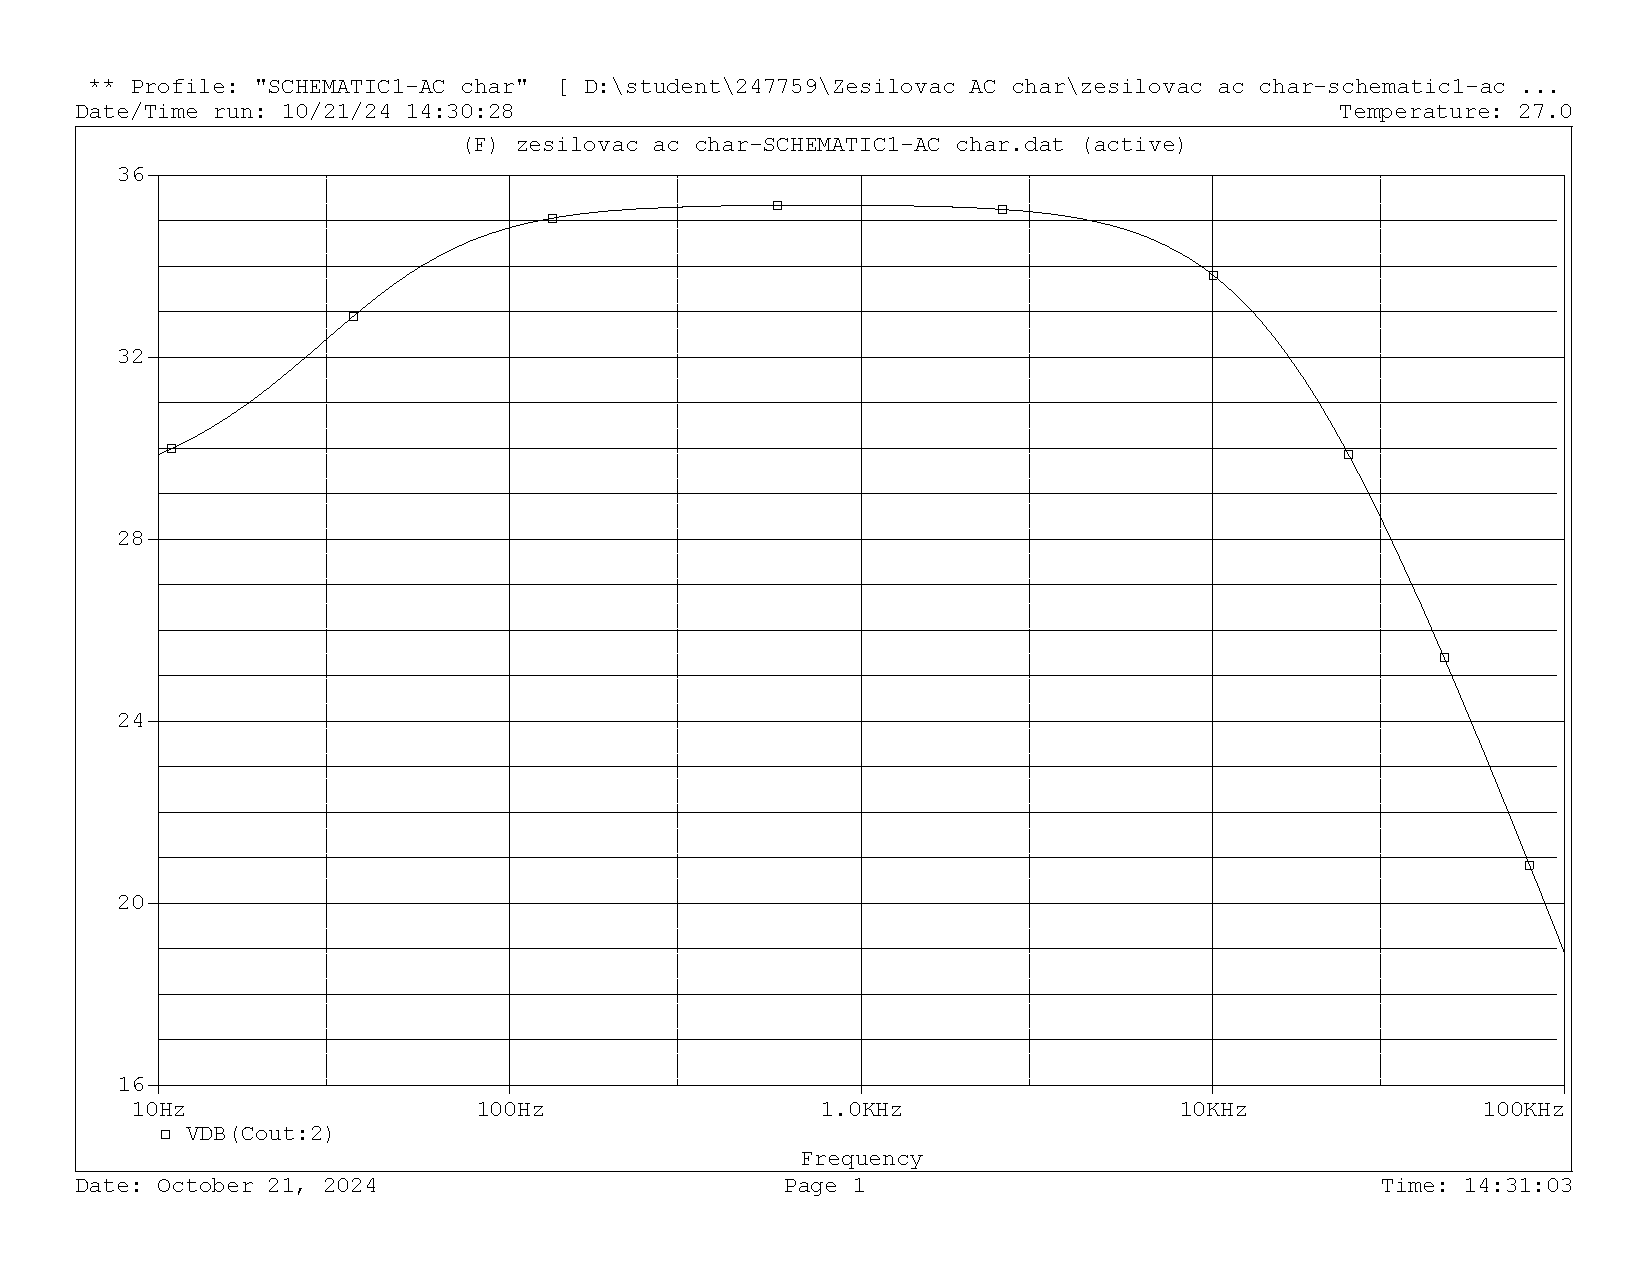
\includegraphics[width=\textwidth]{charakteristiky/uloha3_Ck_5krat_vetsi_5u.pdf}
        \caption{Pětinásobek původní hodnoty Ck (5 $\mu$F)}
    \end{subfigure}
    \hfill
    \begin{subfigure}{0.49\textwidth}
        \centering
        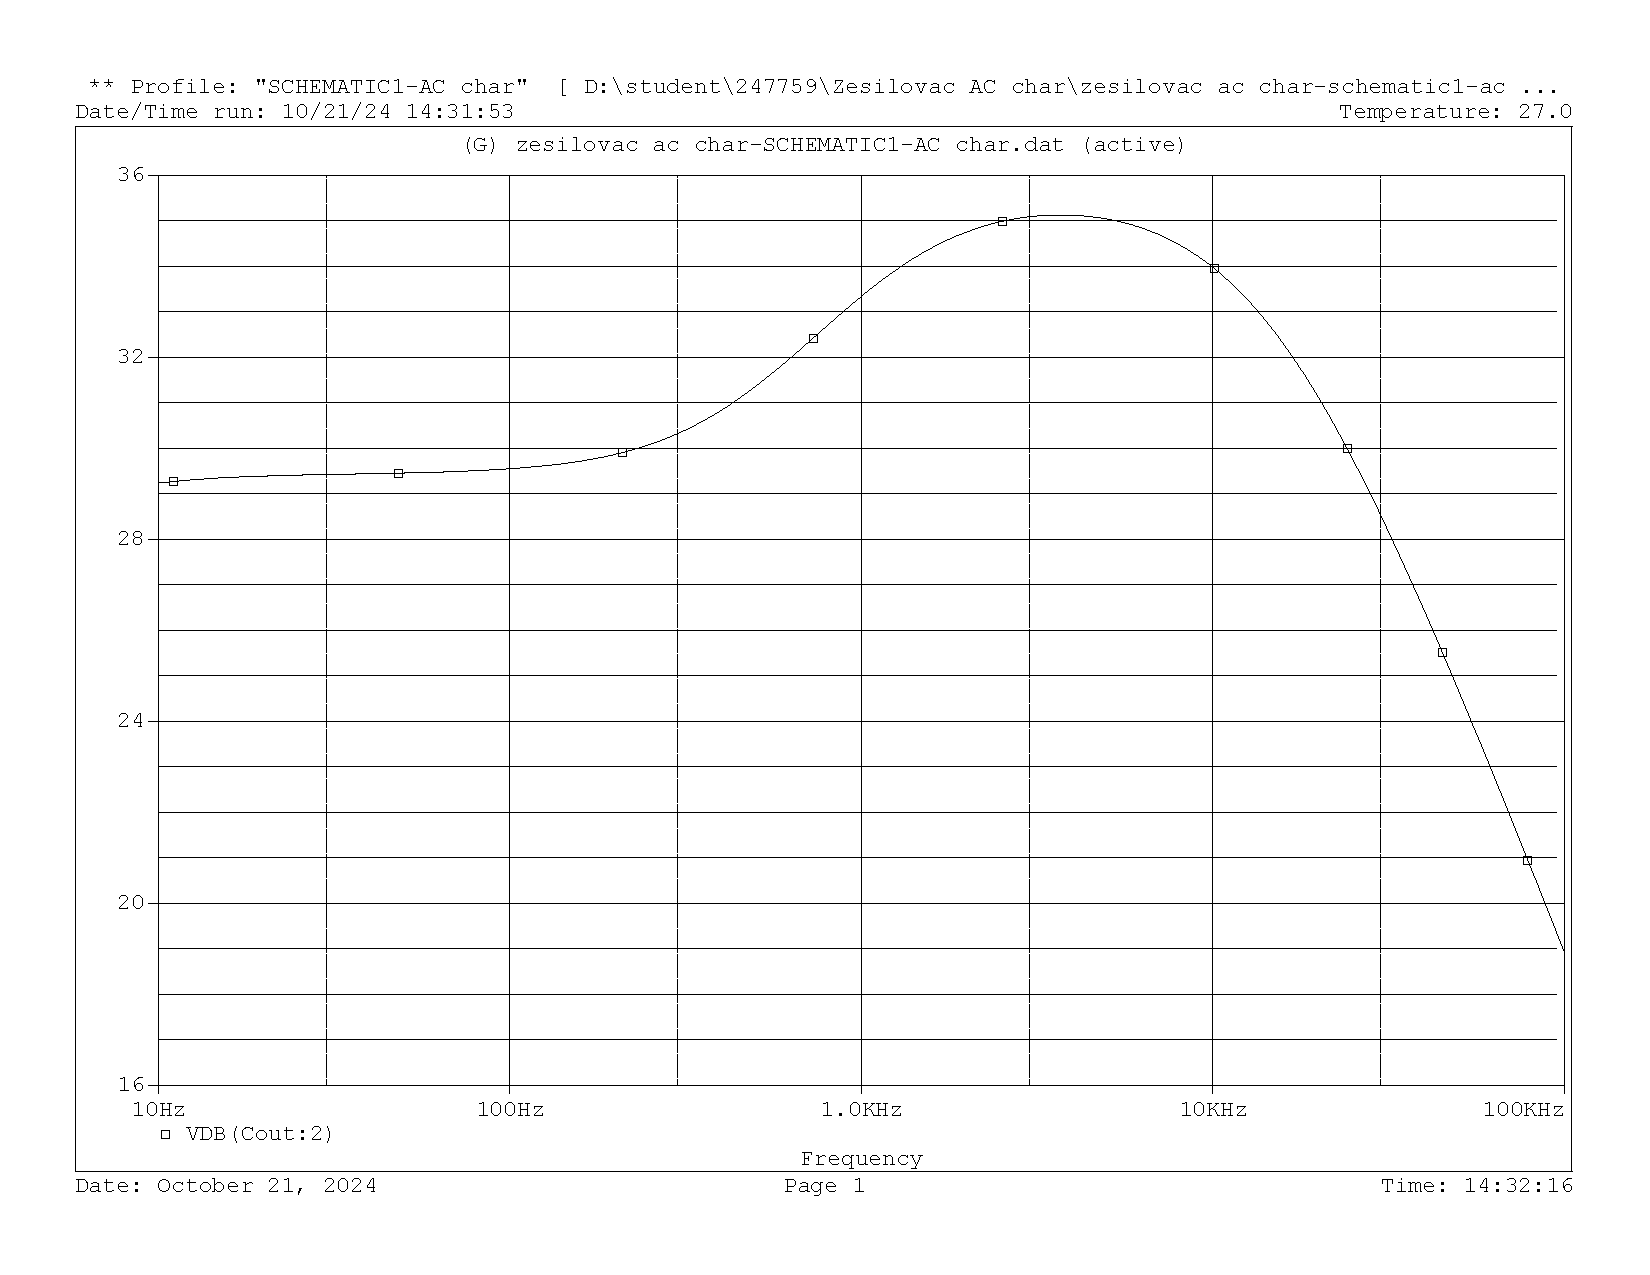
\includegraphics[width=\textwidth]{charakteristiky/uloha3_Ck_5krat_mensi_0_2u.pdf}
        \caption{Pětina původní hodnoty Ck (0,2 $\mu$F)}
    \end{subfigure}
    \caption{Vliv hodnoty katodového kapacitoru Ck na průběh zesílení}
\end{figure}

Změnou hodnoty katodového kapacitoru Ck pozorujeme posun přechodového kmitočtu horní propusti, která omezuje zesílení v nižších kmitočtech.
Nedochází zde však k úplnému potlačení přenosu, což je způsobeno právě CR články na vstupu a výstupu obvodu.

\begin{figure}[H]
    \centering
    \begin{subfigure}{0.49\textwidth}
        \centering
        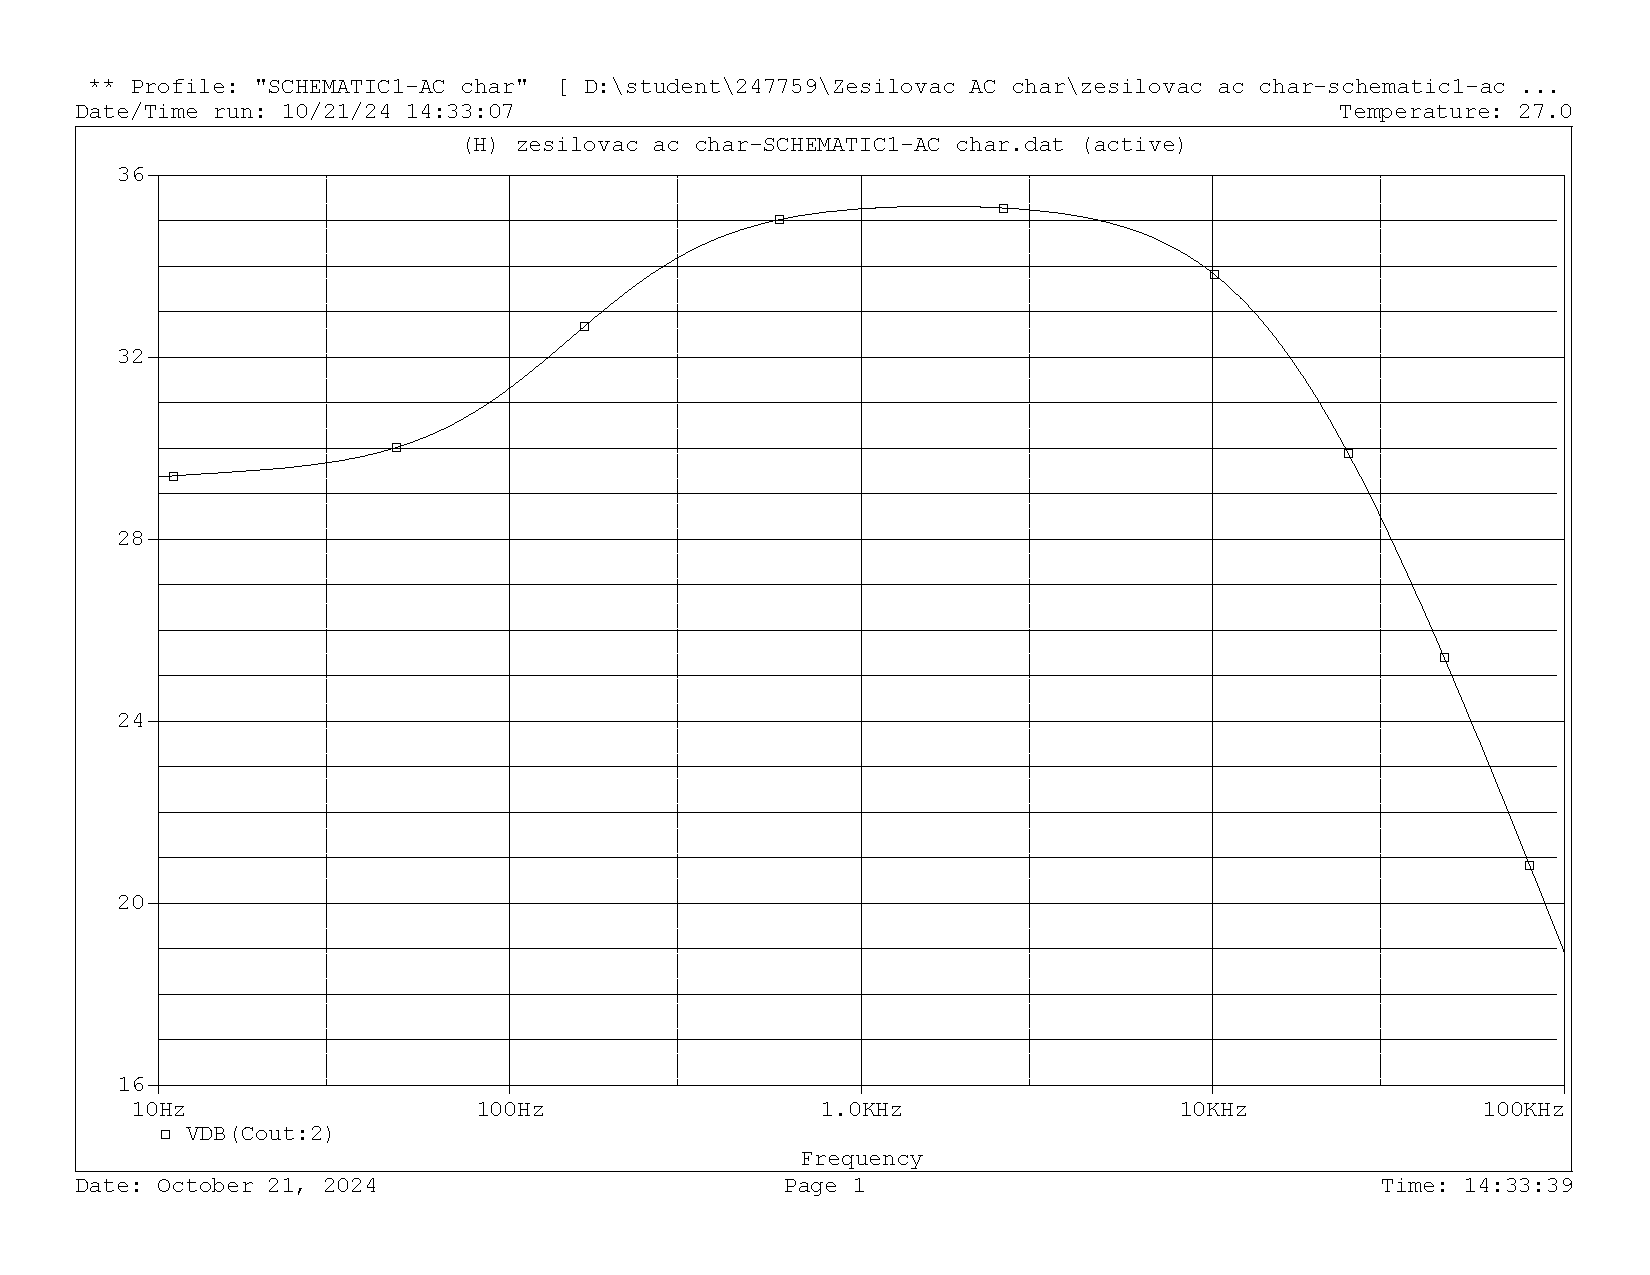
\includegraphics[width=\textwidth]{charakteristiky/uloha3_Cin_5krat_vetsi_500n.pdf}
        \caption{Pětinásobek původní hodnoty Cin (500 nF)}
    \end{subfigure}
    \hfill
    \begin{subfigure}{0.49\textwidth}
        \centering
        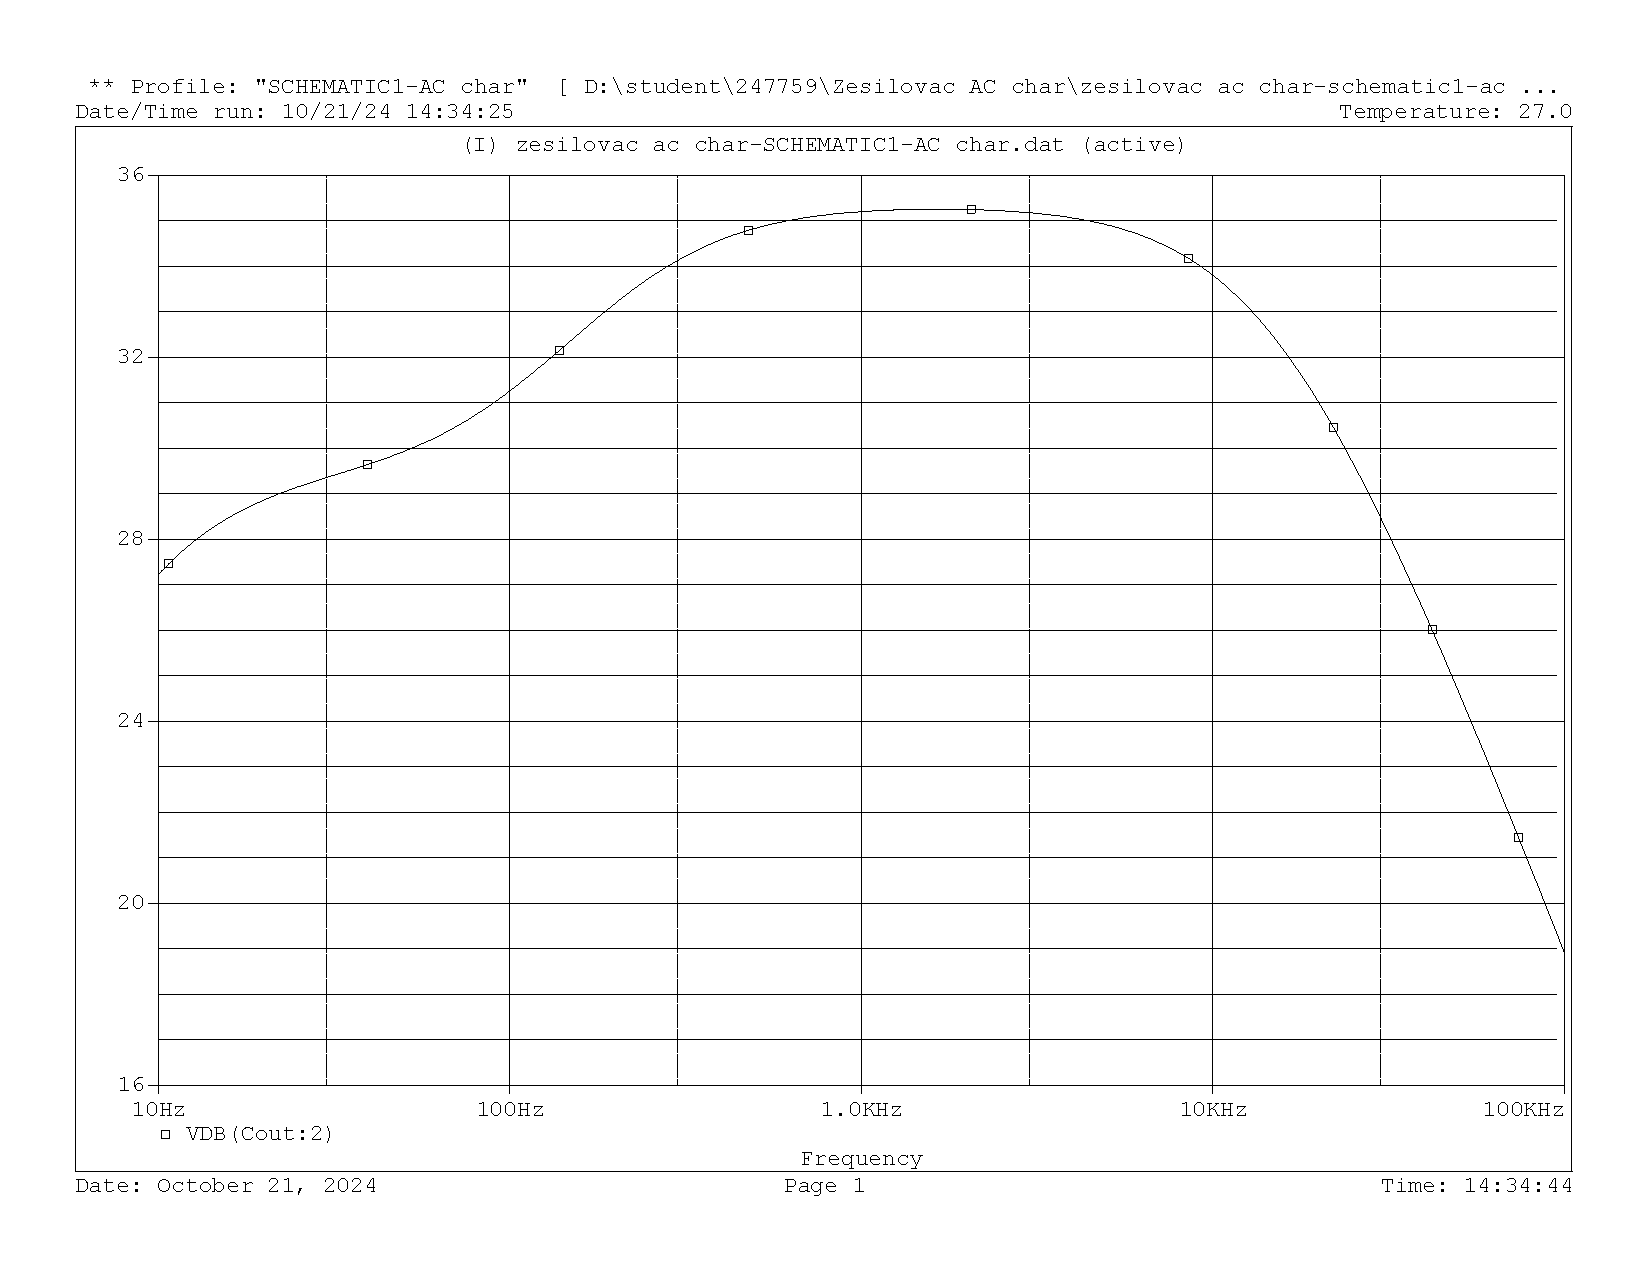
\includegraphics[width=\textwidth]{charakteristiky/uloha3_Cin_5krat_mensi_20n.pdf}
        \caption{Pětina původní hodnoty Cin (20 nF)}
    \end{subfigure}
    \caption{Vliv hodnoty vstupního vazebního kapacitoru Cin na průběh zesílení}
\end{figure}

Změnou hodnoty vazebního kapacitoru Cin pozorujeme posun přechodového kmitočtu horní propusti, která omezuje zesílení v nejnižších kmitočtech na počátku charakteristiky.
Tento jev je zejména patrný při snížení kapacity, viz. obrázek (b).

\begin{figure}[H]
    \centering
    \begin{subfigure}{0.49\textwidth}
        \centering
        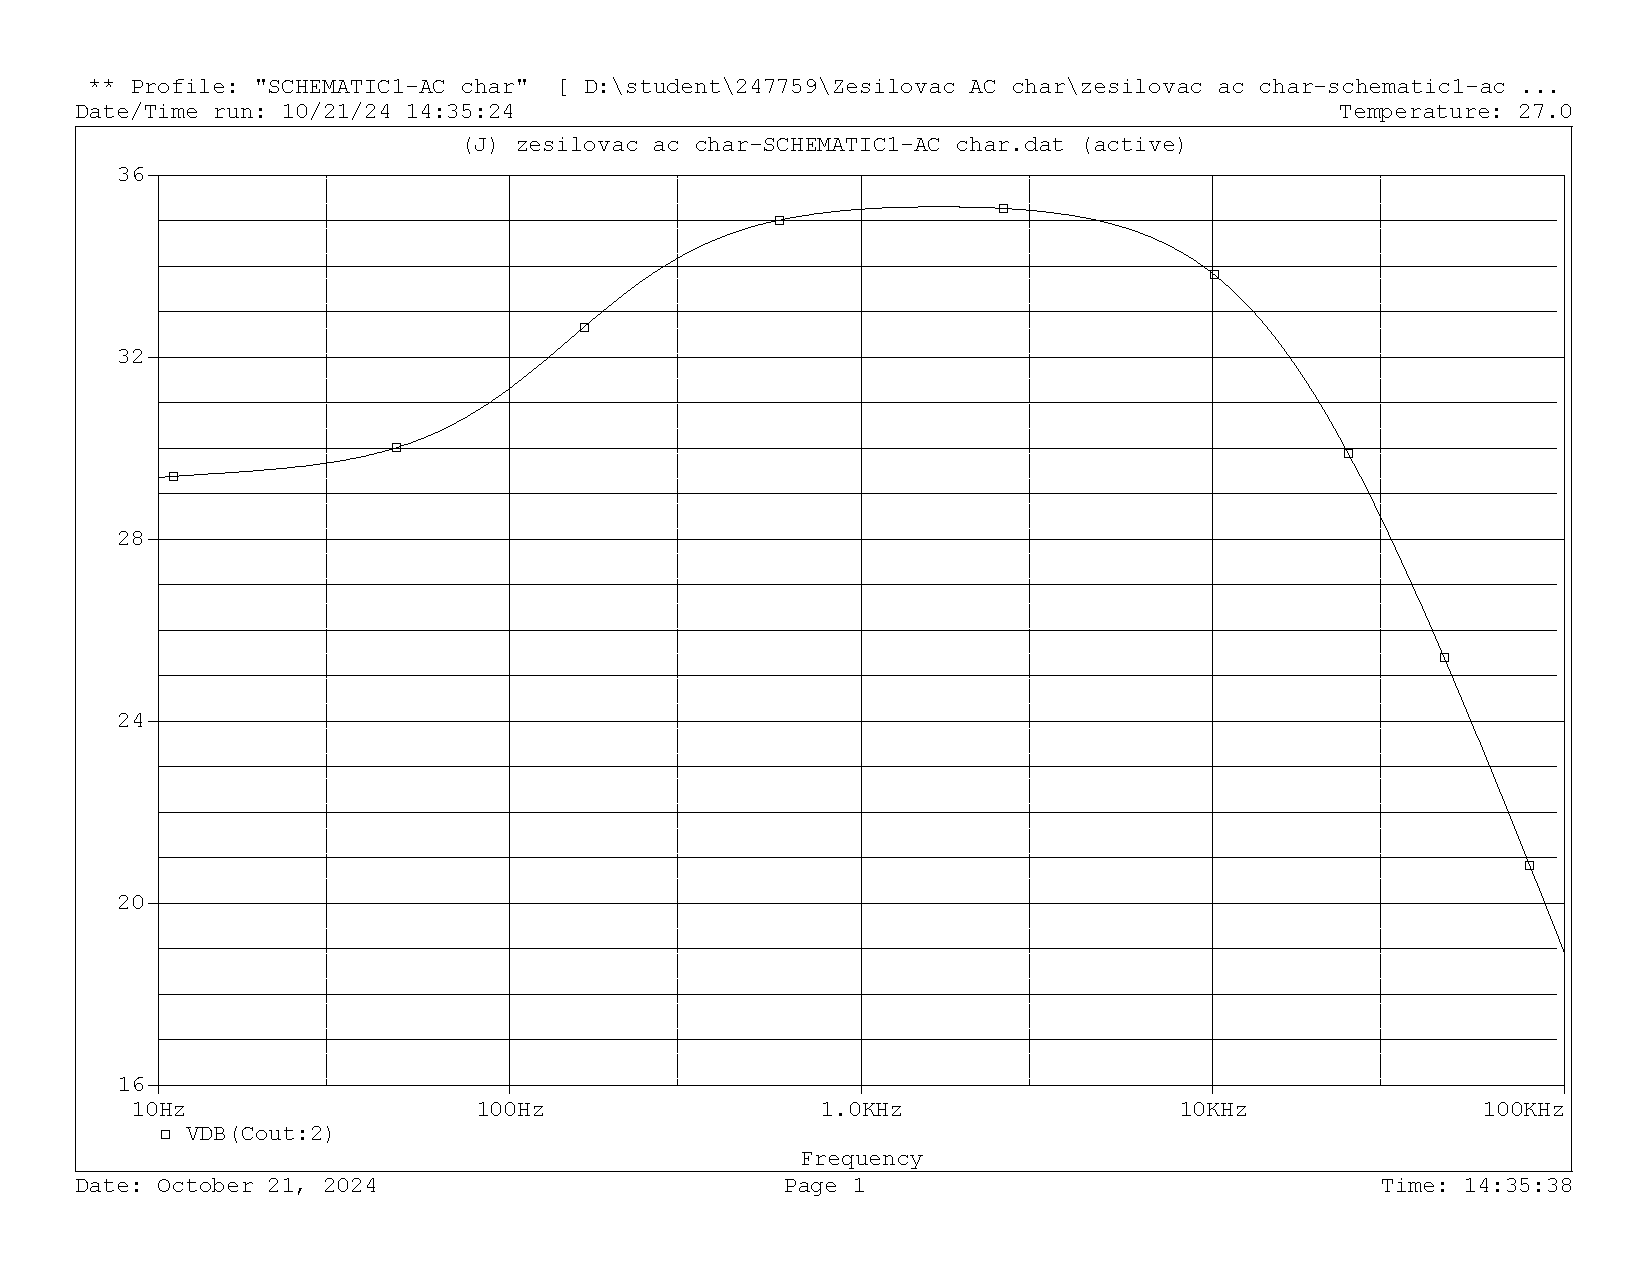
\includegraphics[width=\textwidth]{charakteristiky/uloha3_Cout_5krat_vetsi_500n.pdf}
        \caption{Pětinásobek původní hodnoty Cout (500 nF)}
    \end{subfigure}
    \hfill
    \begin{subfigure}{0.49\textwidth}
        \centering
        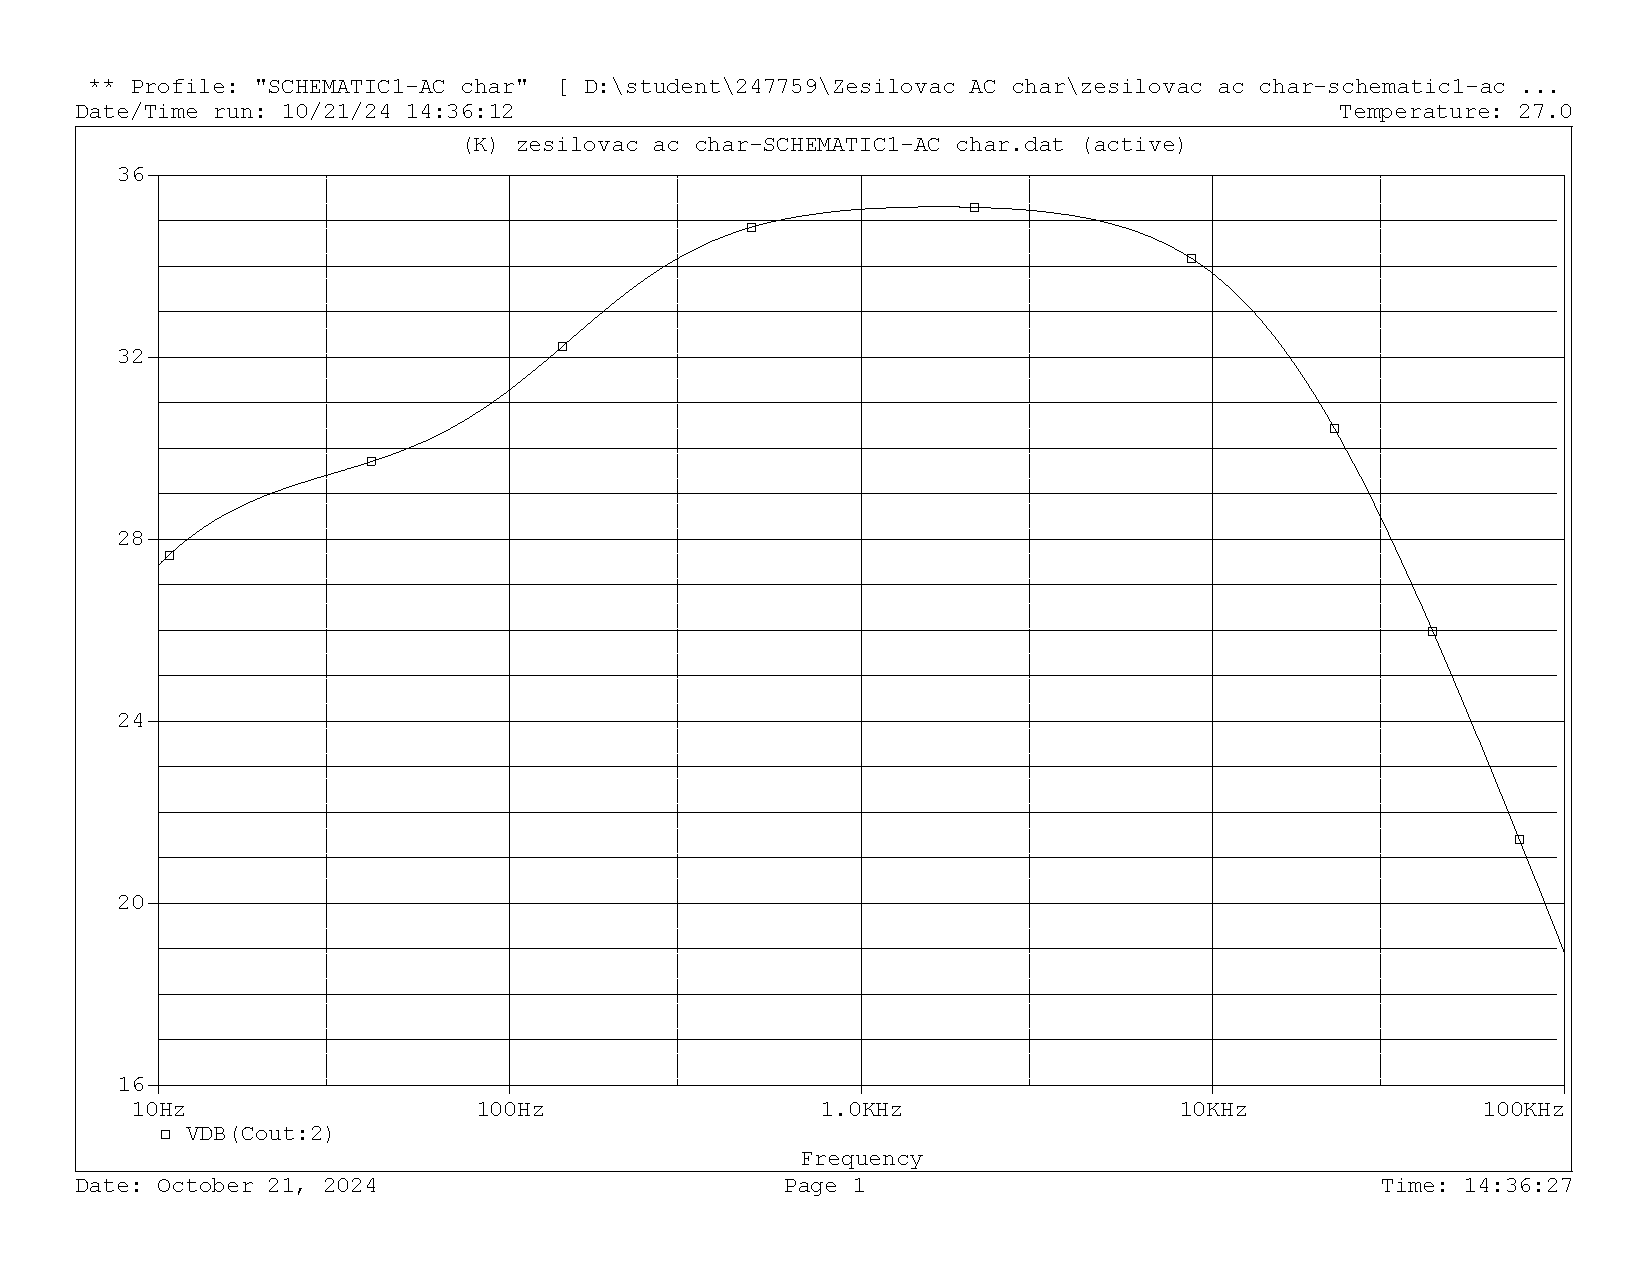
\includegraphics[width=\textwidth]{charakteristiky/uloha3_Cout_5krat_mensi_20n.pdf}
        \caption{Pětina původní hodnoty Cout (20 nF)}
    \end{subfigure}
    \caption{Vliv hodnoty výstupního vazebního kapacitoru Cout na průběh zesílení}
\end{figure}

Změna hodnoty vazebního kapacitoru Cin má za následek téměř totožný efekt, jako změna vstupního vazebního kapacitoru Cin uvedena výše.
To je způsobeno tím, že na vstupu a výstupu se nachází stejný CR článek, takže totožné změny jako v předchozím bodu mají za následek totožný jev.

\pagebreak

\subsection{Úkol měření 4)}

V tomto úkolu jsme se věnovali simulaci časových průběhů sinusových signálů v obvodu.

\begin{figure}[H]
    \centering
    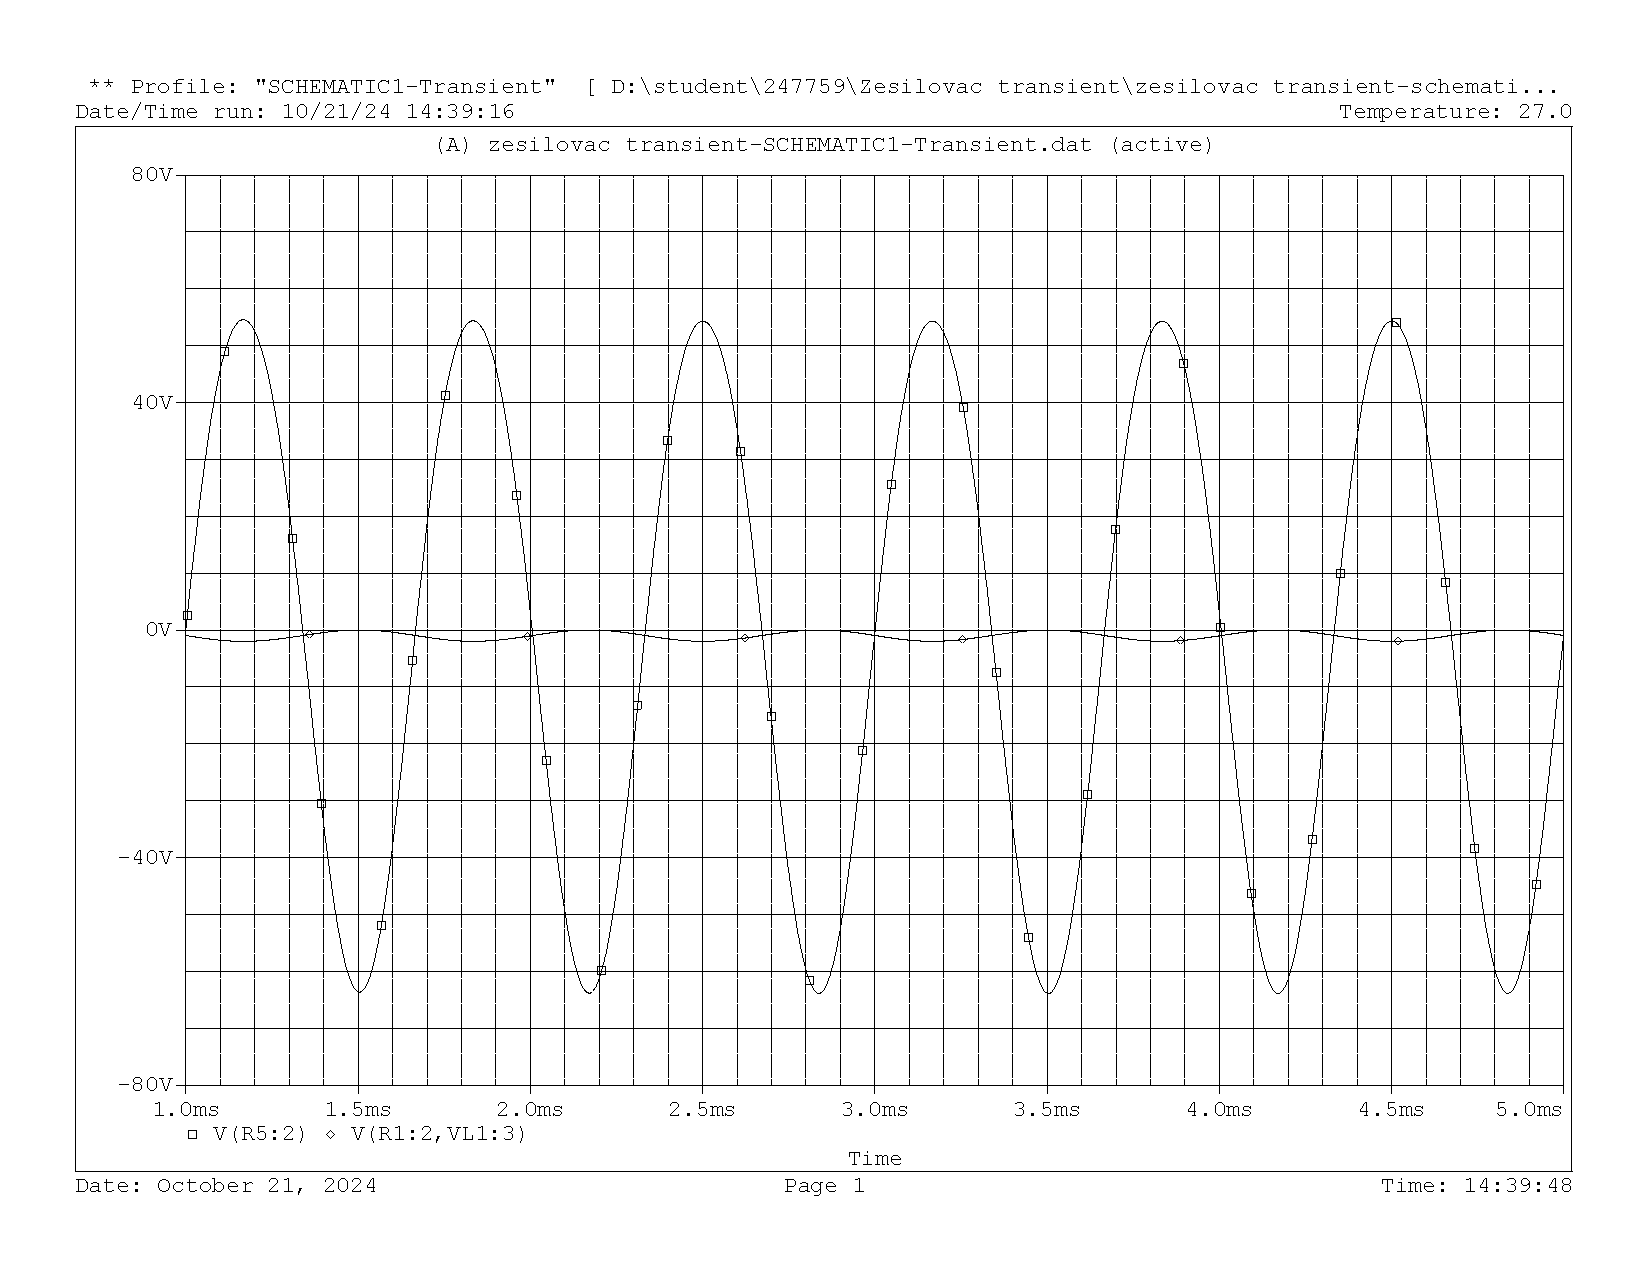
\includegraphics[width=\textwidth]{charakteristiky/uloha4.pdf}
    \caption{Časový průběh signálu v obvodu}
\end{figure}

Zde pozorujeme velmi patrné zesílení výstupního signálu oproti vstupnímu.
Vstupní signál je stejnosměrně posunut do záporných hodnot, jelikož se tam nachází pracovní bod elektronky, která má mřížku řízenou záporným napětím.

\begin{figure}[H]
    \centering
    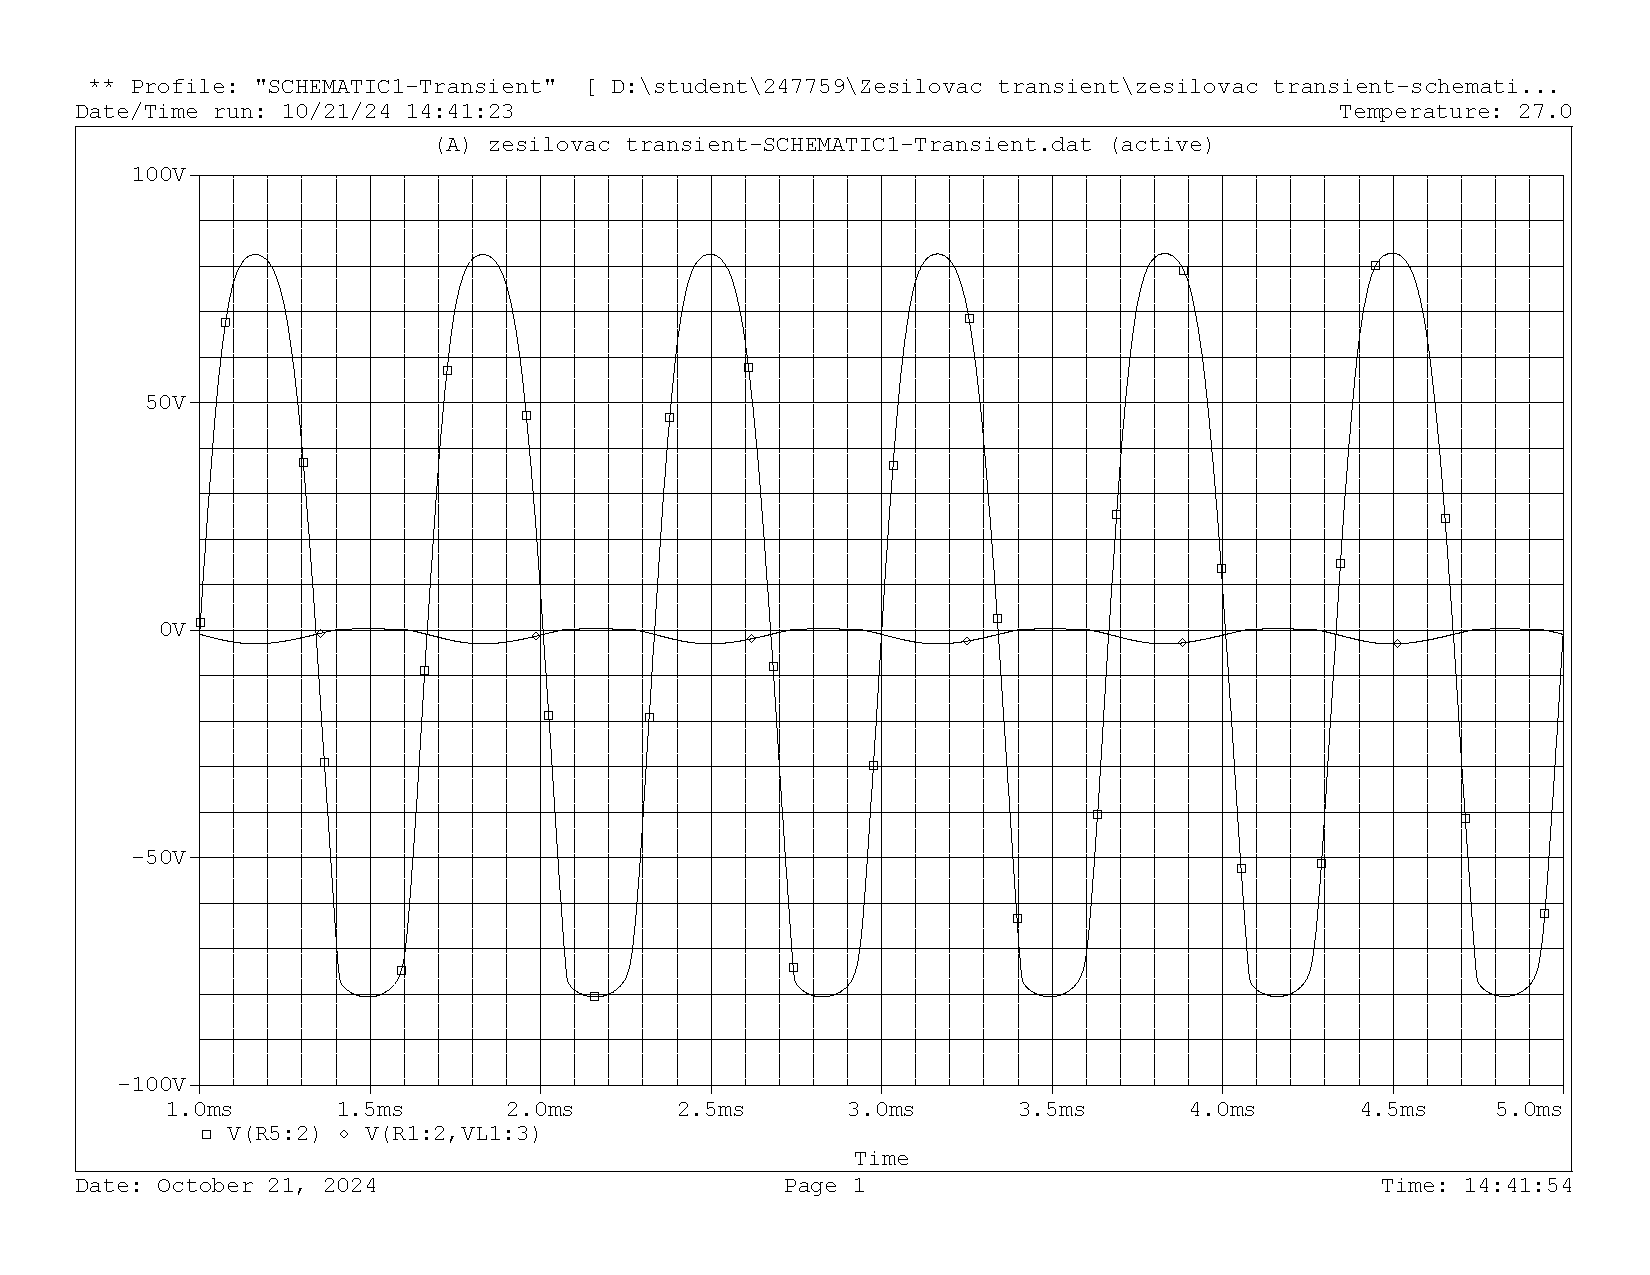
\includegraphics[width=\textwidth]{charakteristiky/uloha4_2v.pdf}
    \caption{Časový průběh signálu se zvýšenou amplitudou s patrnou limitací}
\end{figure}

Pokud zvýšíme amplitudu vstupního signálu na hodnotu 2V, tak začne docházet ke zkreslení signálu v jeho kladných i záporných vrcholech.

Zkreslení kladných vrcholů signálu je způsobeno tím, že vstupní signál přiveden na mřížku s rozkmitem vyšším než 0V už nijak dále nemůže přispět k většímu otevření triody, která je otevřena maximálně.
Dochází zde tedy k limitaci signálu.

Zkreslení záporných vrcholů signálu je způsobeno nelinearitou chování triody v této napěťové oblasti (viz. převodní charakteristika v úkolu č.1).
Dále však dochází k limitaci signálu i zde, jelikož trioda se při příliš nízkém napětí na mřížce uzavírá a nedochází k přenosu signálu.

\pagebreak

\subsection{Úkol měření 5)}

V posledním úkolu jsme se věnovali výpočtu harmonického zkreslení THD při vstupní amplitudě signálu 2V z prvních dvaceti harmonických složek signálu.
Pro odečtení velikosti jednotlivých harmonických složek byla použita Fourierova transformace.

\begin{table}[H]
    \catcode`\-=12
    \centering
    \caption{Velikosti amplitud jednotlivých harmonických složek výstupního signálu}
    \begin{tabular}{ccc}
        \toprule
        $n$       & $f$         & $U_n$      \\
        \cmidrule(rl){1-3}
        [-]       & [kHz]       & [V]        \\
        \midrule
        1         & 1,5         & 91,00      \\
        2         & 3,0         & 1,047      \\
        3         & 4,5         & 11,07      \\
        4         & 6,0         & 2,828      \\
        5         & 7,5         & 0,369      \\
        6         & 9,0         & 1,040      \\
        7         & 10,5        & 1,065      \\
        8         & 12,0        & 0,389      \\
        9         & 13,5        & 0,250      \\
        10        & 15,0        & 0,411      \\
        11        & 16,5        & 0,275      \\
        12        & 18,0        & 0,121      \\
        13        & 19,5        & 0,168      \\
        14        & 21,0        & 0,166      \\
        15        & 22,5        & 0,112      \\
        16        & 24,0        & 0,074      \\
        17        & 25,5        & 0,100      \\
        18        & 27,0        & 0,088      \\
        19        & 28,5        & 0,048      \\
        \bottomrule
    \end{tabular}
\end{table}

Počet námi odečtených harmonických složek během měření je devatenáct místo zadaných dvaceti z toho důvodu, že neumíme počítat.
Dopustili jsme se tedy systematické chyby měření.
Jelikož je ale poslední harmonická složka (kterou jsme neodečetli) velmi malá, a tím pádem i její vliv na výsledek je malý, tak výsledná odchylka výsledku bude také poměrně malá.

\begin{equation*}
    THD = \sqrt{\frac{U_2^2 + U_3^2 + ... + U_{20}^2}{U_1^2 + U_2^2 + ... + U_{20}^2}} \cdot 100 \% = \underline{\underline{12,64\ \%}}
\end{equation*}

Tento výpočet byl proveden v programu Microsoft Excel.
Vliv takto vysoké hodnoty THD na zvuk je velice negativní a nejspíše by způsobil nepřirozeně a nepříjemně znějící hudbu nebo mluvené slovo.

\section{Závěr}

V této úloze jsme se věnovali simulacím zapojení s elektronkovou triodou typu 12AX7.
Nejprve jsme realizovali simulace převodních a výstupních charakteristik triody, díky nímž jsme se seznámili s funkcí a chováním této součástky.
Dále jsme si vyzkoušeli simulaci zapojení elektronkového zesilovače, prozkoumali jeho kmitočtovou charakteristiku a seznámili jsme se s efektem jednotlivých součástek obvodu na průběh kmitočtové charakteristiky.
Nakonec jsme se i podívali jak tato elektronková trioda dokáže zkreslit harmonický signál na vstupu zesilovače, pokud má příliš velkou amplitudu.
Také jsme pomocí Fourierovy transformace určili celkové harmonické zkreslení THD v simulaci.

\end{document}
